\section{Design}
In the implementation, we introduced a concept called grid. A grid was a visual representation of an area (any area) divided into discrete valued cells. The purpose of the grid was to easily view the actual situation and the predicted situation after reconstructing it based on samples from the actual situation (mobile phone sensor readings). As figure \ref{fig:system-overview} shows, we used two separate grids placed next to each other where the left grid is always the actual situation and the right grid is always the predicted situation.
\begin{figure}[here]
  \centering
      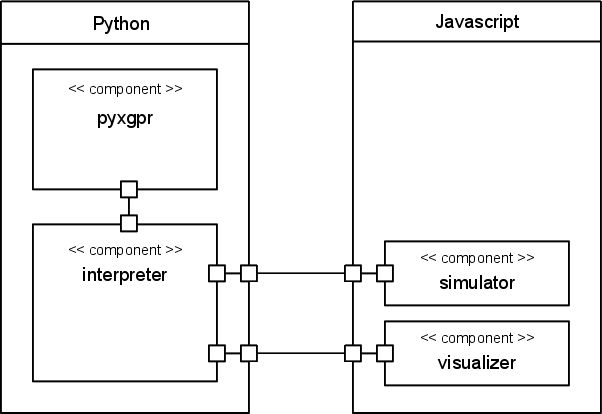
\includegraphics[width=0.7\textwidth]{solution/graphics/system-overview.png}
  \caption{Locates all cells within the boundary.}
  \label{fig:system-overview}
\end{figure}